\openingarticle
\def\ppages{\pagerange{Northwood:firstpage}{Northwood:lastpage}}
\def\shorttitle{Sacred Bodies in Sacred Spaces}
\def\maintitle{Sacred Bodies in Sacred Spaces: Investigating whether western body theory is a valuable tool for interpreting Hindu ritual space}
\def\shortauthor{Lucy Northwood}
\def\authormail{norlu043@student.otago.ac.nz}
\def\affiliation{University of Otago}
\def\thanknote{\footnote{Lucy Northwood recently completed her BA(Hons) degree majoring in archaeology at the University of Otago, New Zealand. Her research interests include the cross over between anthropology and archaeology, religion studies, mind and body theory, pottery, and art and 	iconography. In her spare time Lucy enjoys reading, walking, yoga and daydreaming about travel (as a student, this is often as good as it gets). In 2016, Lucy will continue her studies at the University of Otago and will begin a Master of Arts degree.}}
%--------------------------------------------------------------
\mychapter{\maintitle}
\begin{center}
	{\Large\scshape\shortauthor \thanknote}\\[1em]
	\email \\
	\affiliation
\end{center}
\vspace{3em}
\midarticle
%--------------------------------------------------------------
\label{Northwood:firstpage}
	%----------------------------------------------------------------------------------------
	\begin{myabstract}
Western \marginnote{Abstract} constructs of the mind and body duality have left archaeologists inadequately equipped to appreciate Hindu sacred spaces and bodily practices. As a result, a great deal of the archaeological literature that concerns Hinduism is often based on a political or architectural framework, which bypasses personal devotion and the ritual practices that are fundamental to Hindu religious beliefs. In order to overcome this limitation in archaeological theory, it is proposed that Hindu bodily practices need to be removed from western understandings of the body and placed within their own theological context. Looking to other disciplines for sources of knowledge will not only enrich archaeological accounts of ritual landscapes, but will also provide a more nuanced and reflexive view of Hindu ritual practices.

\keywords[Keywords]{South Asia, mind and body theory,phenomenology, social archaeology, Hindu theology.}
\end{myabstract}

\lettrine[nindent=0em,lines=3]{W}{estern} theory has not only limited archaeological understandings of the body, but also the embodied relationships with material culture and ritual landscapes that are intrinsic to religious bodily practice \parencite{Hamilakis_2002, Insoll_2004}. Contemporary sociological and philosophical understandings of the body \parencites{Bourdieu_1977}{Foucault_1977} have influenced archaeologists to interpret past bodies as a tool, that are often used to visually reconstruct narratives of economy, power and gender \parencites{Barrett_1994}{Shanks_1987}. As a result, many archaeological explanations of religious practices and identity have become rigid through the application of a purely western interpretation \parencites{Edwards_2005}{Insoll_2004} . However, this article proposes that a multi-disciplinary approach, which draws on theological and archaeological knowledge, can provide an alternative understanding of lived and embodied experiences. Through a close examination of how western body theory differs from Hindu theological ideas of the divine body, this article will examine the relationship between Hindu cosmology and archaeological landscapes. Using the Babri Masjid as a case study this paper will demonstrate how a more nuanced and holistic approach can grant archaeologists the opportunity to appreciate the depth of contemporary and past Hindu experience  me with the text. You can copy/paste the text of the article. After that try to compile it and see whether you receive errors.
	
%	\section {A history of approaches}
	Western\marginnote{A history of approaches} intellectualism has been preoccupied with studying the products of the mind, and in turn, the mind’s authority over the body \parencites{Butler_1990}{Shilling_1993}{Shilling_2008}. French philosopher, Michael Foucault, was enormously influential in how the body was approached in academic discussion. Foucault envisioned that bodies are a construction of a historically dominant episteme that govern how individuals live their lives \parencites{Boric_2008}{Foucault_1977} . In one of his earlier publications, Discipline and Punishment, \textcite{Foucault_1977}  argues that the body is seen as a passive tool of control, and that constant surveillance of our actions forces us to internalise norms of social behaviour. Foucault stated that our bodies are repressed by our mind, and argues that;
	Our Society is one not of spectacle, but of surveillance… It is not that the beautiful totality of the individual is amputated, repressed, altered by our social order, it is rather that the individual is carefully fabricated in it, according to a whole technique of forces and bodies \parencite [217] {Foucault_1977}.
	Foucault’s pivotal research sparked academic discussions that began to see how the mind fabricated ‘normal’ ideas about the body \parencite{Meskell_1996, Wylie_1992}. \textcite[6]{Cranny-Francis_1995} stated that an isolated focus on the mind has created fixed ideas of the ‘normal body’, the idea that the body is not only male, but also middle-class, heterosexual and from an Anglo cultural background. A critical reassessment of mind theory saw that not only had society engraved an idea of how our minds are superior to our bodies, but also how academia had readily accepted the Cartesian duality of the mind and body \parencites {Meskell_1998}{Yates_1993}.

	Western theoretical discussions of the mind and body duality have continued to be at the forefront of feminist critiques of western academia. Initially, feminist theorists used Foucault’s idea of surveillance to argue that the female body has been constructed as the lesser, inferior tool of the male mind \parencite{Butler_1990}. \textcite [1] {Cranny-Francis_1995} states that female’s roles are not natural, but are culturally constructed and are therefore subject to critique and change. This idea became the basis for the sex-gender distinction, which highlights the idea of gender as a social construction that is mapped and inscribed onto the physical body \parencite [2]{Cranny-Francis_1995}. Feminist critiques of mind and body theory not only highlight the impact of Foucault’s work, but also how easily academia has accepted the ‘normal body’ without question. However, in more recent years, third wave feminist approaches have begun to break down the binary constraints of Foucauldian theory by challenging the idea that women belong to a homogenous group (Butler, 1993). For example, \textcite [59]{Wylie_1992}  states “Feminists can no longer assume substantial commonalities in the power held, exercised, or suffered by women as women.” This idea sought to place bodies, particularly female bodies, in a theoretical realm that broke the constraints of Cartesian and Foucauldian understandings of the body.  As a result, archaeological theorists have begun to approach these unasked questions, and have critically evaluated how social ‘norms’ have influenced archaeological method and theory \parencites{Insoll_2007}{Yates_1993}. 
	\textcite [4]{Boric_2008} point out that the acceptance of the mind and body duality has created an idea of ‘the body as artefact’ and the body as a ‘scene of display’. Across the board, western humanities scholarship has been dominated by ideas of what it means to have a body rather than the repercussions of the mind and body duality \parencite[146]{Shilling_2008}.

	Archaeology often draws on a wide range of philosophical and epistemological theoretical traditions in order to establish past theories of body, space and culture\parencite[16] {Low_2003}. The ‘normal body’ has in turn become a large part of how archaeologists interpret burials and scared landscapes. Archaeological investigations of past bodies are often based on a semiotic approach, where material culture will be interpreted as a direct expression of identity wealth and gender \parencites{Barrett_1994}{Shanks_1987}. The ‘normal body’ has been translated as the ‘inscriptive body’ and is “mainly approached as an objectified entity in physical biological anthropological studies, or, as the dead body of mortuary studies, as an index of social organization, or as a focus of symbolism” \parencite[151]{Joyce_2005}. Archaeological investigations of the body have often determined that the ‘inscriptive body’ can be read and that associated material culture is a symbolic of how that particular body lived. For example, \textcite[114]{Lee_2000} investigated burial textiles in order to interpret gender in Minoan burials, in her research she states “the essential components of dress…emit constant, complex, social messages that would have been intended by the wearer and understandable by the viewer”.\textcite {Lee_2000} case study is an example of the ‘inscriptive body,’ where the body is interpreted as public domain, and a ‘tool’ that is used to express social position, both in life and in death. Although the ‘inscriptive body’ has allowed archaeologists to trace patterns of accumulative wealth, social identity and gender in archaeological societies, the method will often take a two dimensional approach to understanding the past \parencite {Meskell_1996}. The ‘inscriptive body’ is based upon the social construction of the ‘normal body’, which in turn means archaeologists will often reflect their own habitus on to past communities \parencites{Bourdieu_1977}{Comaroff_1989}.

	Over the last thirty years, an increase in academic discussions of the western mind and body duality has started to further influence the methods that archaeologists use to interpret past bodies and communities. Archaeologists are beginning to borrow theoretical frameworks from other disciplines in order to explain phenomena within the archaeological record. At the forefront of this development is phenomenology, an approach that is concerned with embodied experiences of archaeological landscapes \parencites{Copeland_2009}{Tilley_1994}. Phenomenology was developed by German philosopher, Edmund Husserl, as a direct criticism toward mathematical and scientific explanations of nature and lived experience \parencite[321]{Allsobrook_2014}. In archaeology, phenomenological approaches were adapted as a way of moving away from semiotic understandings of the body, and to deconstruct the dualistic ‘normal body’ in archaeological theory \parencite[65] {Bruck_2005}. Phenomenological archaeology moved away from the ‘inscriptive body’ and began to seek understanding of the phenomena of the ‘lived body’. \textcite [139]{Joyce_2005} states that “analysis of the production and experience of lived bodies in the past through the juxtaposition of traces of bodily practices, idealized representation and evidence of the effects of habitual gestures, postures and consumption practices on the corporeal body” allowed archaeologists to move away from two dimensional understandings of the mind and body dualism. Post-processualists have criticised the ‘inscribed body’ and argue that the orthodox model limits past bodies to an object of public site \parencites {Grosz_1994}{Joyce_2005}{Tilley_1994}. In archaeology, phenomenology became an escape from orthodox models of the ‘body as artefact’ that allowed them to move toward more holistic interpretations of past bodies.

	Phenomenological and social archaeological approaches have particularly strengthened our understanding of how past communities experienced cosmic landscapes \parencites{MeskellPreucel_2007}{Tilley_1994}. Archaeologists have not only noted the material and architectural properties of sacred landscapes, but have also started to explain how landscapes themselves can shape the lived experiences of past bodies.\textcite[199]{Ashmore_2010} describes ceremonial landscapes as an arrangement of specific features where the cosmos is situated on earth, and where ritualised movements between landscape features evoke and reinforce understandings of cosmic order. In this regard, theoretical understandings of the body are less focused on representation and symbolism, and instead on how people lived and experienced cosmic order through their surrounding landscapes. Phenomenological archaeology has however been met with criticism. For example,\textcite [271]{Fleming_2006} questions if phenomenological archaeologists can detach themselves as the ‘observer of past communities’. In regards to cosmic landscapes, it is possible that archaeologists use personal embodied experiences of the cosmos to explain how past communities experienced the sacred. This matter has been particularly questionable in Hindu India, where sacred landscapes have been interpreted as political and symbolic \parencites{Fritz_1986}{Mack_2004}{Sinopoli_2010}. Phenomenology has improved how archaeologists look at sacred landscapes, but these archaeological interpretations will often lack the narratives that are available to them in Hindu theology.

%	\section {Western interpretations of Hindu ritual space}
	In her \marginnote{Western interpretations of Hindu ritual space} 2010 article, \citetitle{Sinopoli_2010}, Sinopoli looked at architecture for information on the construction of an imperial identity within the 14th century southern Indian empire Vijayanagara (Fig. \ref {fig:Northman_fig1}1). Archaeologists will often look at architecture to interpret not only information about the social, political and economic organization of past societies, but also about how social organisation was constructed by the ruling elite\parencite [222]{RenfrewBahn_2012}. \textcite {Sinopoli_2010} argues that Vijayanagara is a sacred landscape, and that the sacred architecture is an amalgam of Islamic, Vedic and local Hindu styles. Although the kings themselves affiliated themselves with The Ramayana, they also followed the Vaishnava sect, which was associated with a monotheistic god who had power over the land and legitimised their right to rule. However, public temples were dedicated to the Vedic goddess Pampa, and Valmiki’s The Ramayana -- a volume of Sanskrit epic poems -- was a large part of temple architecture and worship. \textcite[457] {Sinopoli_2010}  argues that the elite put aside their own religious affiliation in order to pay homage to the religious beliefs of the people. Although \textcite {Sinopoli_2010}makes references to the theological aspects of Indian life, she notes that religion was manipulated by the elite in order to legitimise their right to rule.\textcite {Sinopoli_2010}  outlines a political understanding of Vijayanagara that does not reference how the civic centre was in fact experienced as a cosmic landscape. Although architectural and power based understandings of past Hindu society have been successful in their depiction of the past \parencites{Fritz_1986}{Mack_2004}{Sinopoli_2010}, there has not yet been enough research that maximizes the potential of past Hindu narratives. Archaeologists have often favoured systematic understandings of Hindu landscapes, without engaging with the theological narratives that are available to them \parencite {Sugandhi_2011}. Hindu landscapes are often underrepresented and misunderstood because of the western dualistic understanding of the mind and body relationship.
	
\begin{figure}[!htb]
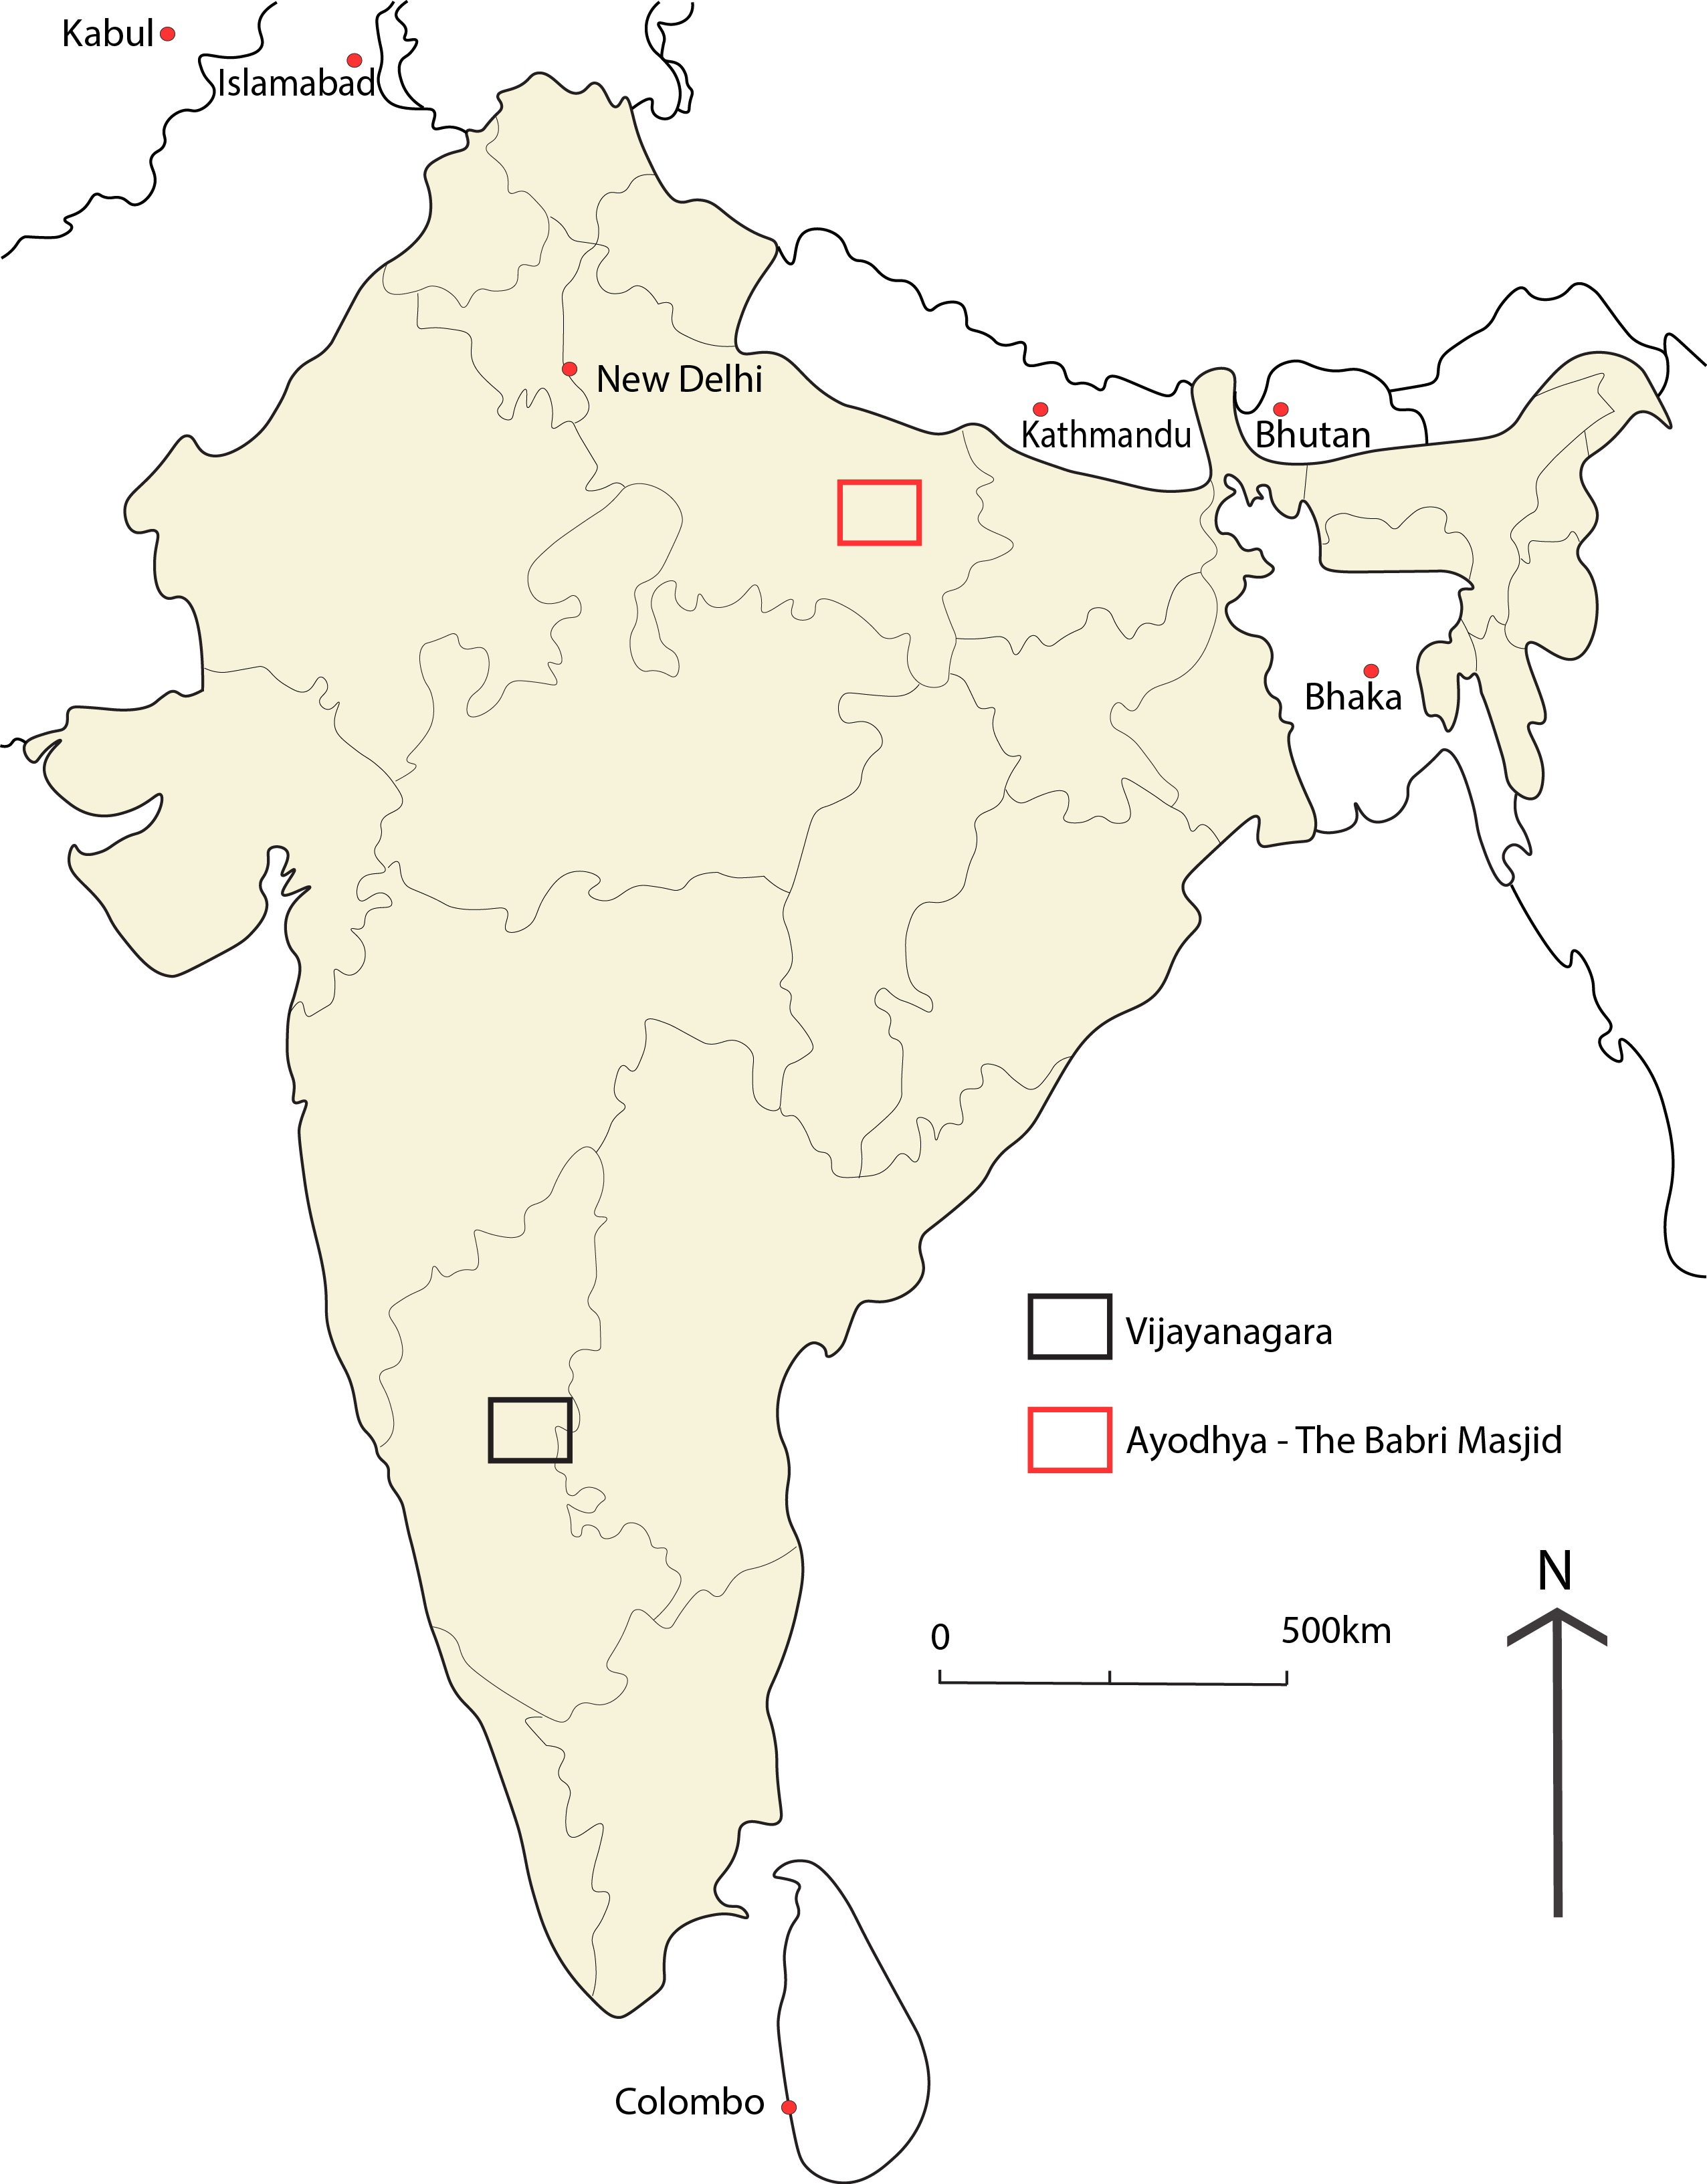
\includegraphics[width=\linewidth]{figures/Northman_fig1}
\caption{Map of India}
\label{fig:Northman_fig1}
\end{figure}
	 
%	 \section {Hindu theological understandings of the body}
In order\marginnote{Hindu theological understandings of the body} to reach a multi-dimensional understanding of Hindu cosmic landscapes, it is important to consider Hindu theological understandings of the body. Western body theory is not universal, and perspectives of the body are interchangeable according to different religious and cultural communities. In Hinduism, body theory is shaped by theological ideas of divine embodiment \parencite {Beck_1976}. The gods are present in all aspects of Hindu life, and are often depicted in village temples, family homes and on the roadside. These images – most often called murtis – are one of the few ways in which the divine become manifest in Hindu daily life. Although the divine is thought of as a formless, bodiless, and absolute being, the divine can also transcend into an earthly form. The idea that the divine are formless, and that they have form, happily co-exists in Hindu religious theory \parencite[211] {Smith_1989}. In Hindu traditions, the principle underlying divine embodiment stems from the idea of the avatara – meaning descent – and underlines the descent of a god into the world. This theology was formulated in the Bhagavadgita, where the avatar of Vishnu was said to “create myself ... [and] take on existence from eon to eon, for the rescue of the good and the destruction of evil” \parencite[87] {Buitenen_1981}. The fluidity of Hindu ideas of the divine, mean that the gods can remain tangible and otherworldly whilst frequently transcending into the physical human realm.

	 In turn, Hindu ideas of the divine mean that Hindu body theory, and perspectives of the self, are entirely different from its western counterpart. For example, western theory considers the mind and body to be entirely separate, whilst in Hinduism there is no distinction between the mind and the body. Like the divine body, the Hindu body can take on multiple forms so that it can move easily between the physical and cosmic realms. The earliest example of the Hindu mind and body as multiple is documented in the Upanishads, a collection of philosophical Vedic scriptures which discuss the fundamentals of Hindu theology \parencite [33] {Patrick_1998}. In the Upanishads, the atman – one’s inner essence – and the Brahman – meaning both the creator and the essence of the universe – are thought to be the same transcendent being \parencite [61] {Staal_1993}. One of the core teachings of Hinduism, is the atman-brahman relationship, the act of joining one’s inner essence with the wider cosmos, through acts of dharma (practice) and karma (action). The human body is therefore believed to have both subtle and gross dimensions and the relationship between the human body and the ritual body is ultimately limitless \parencite {Holdrege_2007}. Therefore, there is no distinction between the mind and the body, as both work in unison and allow the body and the cosmos to intertwine on a daily basis. Hindu body theories are heavily based on theological ideas of divine embodiment and are therefore entirely separate from western ideas of a mind and body duality.

	 Hindu body theory has heavily influenced the way that Hindu communities experience sacred landscapes. The fluidity between the Hindu mind and body means that the divine can transcend into the world at any time. This is most evident in sacred landscapes, where Hindus will go to experience the divine. \textcite[214]{Beck_1976} states that in temple worship, the individual joins with and even becomes identical to the cosmos itself. For this reason, Hindu communities will go on pilgrimage, or visit sacred landscapes so that their atman may merge with the cosmic brahman. Hindu temples will be architecturally designed to maximise the transcendence of the divine into the physical world. For example, the temple foundation of Madurai, an archaeological city in Tamil Nadu, was designed as a replica of the cosmos, so that worshippers could come and experience the earthly dwelling of the divine \parencite [236] {Beck_1976}. The fact that the Hindu body engages with the cosmic has often been over looked by western theorists, and most particularly by archaeologists. The engagement of the human body and divine body in sacred landscapes has either been misinterpreted or misunderstood as ‘Hindu bodily narcism’ \parencite [55] {Smith_1989}. In turn, this means that archaeological interpretations of sacred Hindu landscapes have taken on either a predominantly political or symbolic format \parencites{Fritz_1986}{Mack_2004}{Sinopoli_2010}. If archaeologists wish to interpret sacred Hindu landscapes, then it is essential that they begin to engage with the rich narratives that are available to them.
	 
%	 \section{Case study: Using Hindu theology to understand the conflict surrounding the Babri Masjid}
	 Engaging\marginnote{Case study: Using Hindu theology to understand the conflict surrounding the Babri Masjid} with complex narratives of Hindu theology will not only help archaeologists to interpret sacred landscapes, but also to understand the intrinsic relationship between the contemporary Hindu community and temple architecture. Archaeology has been used as a tool in the religious and political conflict of the Babri Masjid-RamJanmabhumi temple in the Tamil city, Ayodhya (Fig.\ref {fig:Northman_fig1}1). The Babri Masjid was erected during the reign of the first Mughal emperor, Babar, and has been a place for Muslim worship from the mid-1500s to 1949 \parencite [156] {Rao_1994}. However, Hindu nationalists who claimed the Babri Masjid was constructed on the ruins of a Hindu temple contend the mosque, and argue that Muslim nationalists purposefully destroyed Rama’s temple. The Babri Masjid has been the subject of conflict between Muslim and Hindu Indian communities, who each lay claim to the sacred and political elements of the temple. It is important to note here that both sides of the opposition have religious connections to the temple, and have each employed archaeological methods in order to argue their case, but for the purpose of this paper I will discuss the Hindu cosmic relationships with the RamJanmabhumi. The RamJanmabhumi is considered by Hindus to be the birthplace of King Rama, the protagonist and avatara of Vishnu in Valmiki’s sanskrit epic, The Ramayana. The Ramayana did not originate as a religious text, but as an orally transmitted discourse on correct ethical, social and political conduct \parencite[141] {Thapar_1991}. \textcite [143] {Thapar_1991} states that because of this, the Ramayana cannot be placed in a specific time period because the epics were a part of an ongoing tradition that saw them transform from bardic literature to religious scripture in the hands of the brahman elite. Although this makes the Ramayana hard to place archaeologically, the relationship between Ayodhya and Hindu theology is deeply imprinted. As Rama is the avatara of Vishnu, The Ramajanmabhumi is therefore the birthplace and political legacy of both Rama and Vishnu. As a Hindu sacred landscape, worshippers will visit the Ramajanmabhumi to experience not only Rama, but also the earthly dwelling of Vishnu.

	 There is no empirical evidence that the Babri Masjid was ever built on the ruins of a Rama temple \parencite [122] {Bhattacharya_1991}. Both Hindus and Muslims have turned to textual and scientific evidence in order to validate their political claims to the sacred space \parencite [156] {Rao_1994}. Archaeology has been employed by both sides, both of which have used the social science as a means of attaining empirical evidence that claims political authority over the temple. At the forefront of the archaeological debate has been B. B. Lal, the retired Director General of the Archaeological Survey project and head of the ‘Archaeology of the Ramayana’ sites project \parencite [148] {Barber_2006}. \textcite [119-123] {Lal_2001} argued that ‘brick built bases’ and ‘fourteen non-Islamic black basalt pillars’ predated the Babri Masjid and were of Hindu origin. Lal interpreted the evidence with a Hindu perspective, which was met with criticism from Ram Sharma, who argued that the recovery of glazed Islamic pottery from above and below the temple foundations, suggests that the ‘brick built bases’ had collapsed by the time the mosque was constructed \parencite [132-134] {Sharma_2001}. The conflict at Babri Masjid - Ramjanmabhumi not only shows how systematic archaeological evidence can be used as ‘evidence’ in support of a political agenda, but also of how archaeological investigations have separated the temple from its embodied connections with the cosmic realm. The archaeological concern with empirical evidence has over ruled any religious claims of embodied experience with the temple. In Hindu theology, emphasis is placed on orthopraxy rather than on orthodoxy, which means that the Ramjanmabhumi is an important place to practice dharma \parencite[70]{Staal_1993}. Unlike many western religious traditions, Hindus regard the practice of dharma and karma with higher value then religious scripture or scientific evidence. The tendency for archaeology to confront religious and political conflict with empirical evidence often means that the religious narrative becomes neglected or lost.
	 
%	 \section{Avenues for the future} 
Unlike \marginnote{Avenues for the future} western culture, Hindu theology has multiple explanations and manifests for the body, which can be placed in both a divine and physical realm \parencite {Holdrege_2007}. Whilst heavily documented in religion studies and historical accounts of Hindu bodily worship \parencites{Beck_1976}{Smith_1989}{Staal_1993}, archaeological research is yet to explore the transcendence of the Hindu physical body in to the cosmic realm. \textcite[155] {Insoll_2004} argues that narratives of religious experience in archaeology are underrepresented, merely because religion is often considered to be a side note with less importance than studies of society, economics and human migration. However, religious experience can provide a detailed retelling of how people experienced both the physical and cosmological world on a daily basis \parencites{Edwards_2005}{Hamilakis_2002}{Insoll_2004}. Although heavily critiqued \parencite{Fleming_2006}, phenomenological approaches in archaeology highlight that there is a significant gap between human experience and physical landscapes. Phenomenological anthropologists have stated that phenomenology is able to “stress the indeterminate, unarticulated and unbounded nature of experience, which can flow into new meanings and different cultural dynamics” \parencite[50]{Knibbe_2008}. Phenomenologists do however, need to establish themselves as the observer, and need to take a critical position that allows them to acknowledge both the scientific and embodied experiences of sacred landscapes. Similarly, social archaeological approaches have attempted to bring embodied experiences of landscape into archaeological narratives. For example, \textcite {Meskell_1996, Meskell_1998, Meskell_2000}  argues that in order to understand embodied experiences of landscape and material culture, archaeologists need to disregard Foucauldian top-down approaches and turn to methodologies that are multi-disciplinary and culturally sensitive. Through her advocacy for social archaeological perspectives,\textcites{Meskell_1996}{Meskell_1998}{Meskell_2000} argues that archaeologists need to examine archaeological data in its own cultural context, and to refrain from projecting western classifications and body theory on to the human past. In regards to future approaches, Atalay states that archaeologists must “advocate for a collaborative approach that blends the strength of western archaeological science with the knowledge and epistemologies of Indigenous people….We must begin to explore ways of moving beyond posturings that pit science against religion” \parencite [301-302] {Atalay_2006}. Systematic archaeological methods should be used in conjunction with theological narratives in order to provide a richer and more detailed perspective of the archaeological record.

	 Hindu communities bring an alternative perspective to how people see and experience sacred and cosmic landscapes. Western and Hindu theory places the body in completely different contexts, and highlight how communities can see and experience the world in very different ways. Archaeologists have often overlooked these differences, and have provided interpretations based on their own social biases or western interests \parencite {Sugandhi_2011}. If archaeologists are to engage with religious narratives, or past accounts of embodied experience, then it is essential that they employ multi-disciplinary methodologies. For instance, removing Hindu religious practices from binary western interpretations will provide a more reflexive and holistic understanding of past religious practices \parencites{Insoll_2004}{Insoll_2007}. Overall, Hindu bodily experience remains underrepresented in the archaeological record, but there is promising potential to improve how archaeologists approach religious landscapes and material culture. In order to move forward, it is proposed that a more nuanced and reflexive view of archaeological landscapes is required before archaeologists can fully understand Hindu ritual space.
	 \myseparator
%	 \section{Acknowledgements}
	 It\marginnote{Acknowledgements} is fair to say that I would not recognise my own research interests if it weren’t for the University of Otago’s Anthropology and Archaeology department. I owe a very large thank you to Dr. Ian Barber, Dr. Tim Thomas and the fourth year theory class of 2015, without your support and passionate debate I may never have found the courage to submit this paper. I would also like to thank all those involved in the IJSRA. I cannot thank you enough for this entire experience, and for creating a space where students can share the products of their incredible minds and late nights. Finally, I would like to dedicate this article to my late father, Terence Walton, who from a very young age taught me the value of reading, open-minded thinking, laughing until it aches, and Randy Newman. Thanks Dad.
	
	


\printbibliography[heading=subbibnumbered] 
\label{Northwood:lastpage}
\closingarticle

